% Descripción
% La propiedad lógica descripta sólo dice que la imagen resultante va a tener la misma cantidad de pixeles y el mismo ancho, pero no describe la imagen resultante en cuestión, no le veo mucho sentido.
% [DONE] La imagen de la transformación está al revés
% Implementación
% La descripción de qué se hace con los punteros a los cuadrantes necesita una re-escritura.
% El código presentado no es claro, qué tienen r10 y r11?
% Análisis preliminar
% No se explica cómo están hechos los experimentos.
% Cómo hicieron el gráfico? Pusieron todos los datos sobre cada ejecución? El gráfico de esta manera puede dar una idea de la varianza, pero no se sabe bien qué tomaron para armar la recta.
% Hipótesis de trabajo
% [DONE] Las consignas, como "Conjunto de ideas de experimentos" indican qué debe ir (no necesariamente tienen que ser títulos).
% [DONE] La comparación entre ASM y C entra dentro de los análisis preliminares.
% Loop unrolling generalmente es aplicado cuando se tiene una cantidad fija de ciclos. Acá lo que hicieron fue hacer un solo unroll del loop, no?
% Experimentación
% La descripción del experimento que les parece interesante debería ir en un apartado "trabajos futuros". Ahí está un poco descolocado.
% El párrafo que comienza con "El roll del cache en imágenes grandes" debería ser re-escrito, tiene varios errores.
% La explicación de lo que se va a medir, debería ser concisa:
% Queremos medir x cosa (el por qué debería estar claro en la hipótesis del trabajo) y cómo lo vamos a hacer.
% Ejemplo (no es para que lo copien literal): Las mediciones se hicieron con tal mecanismo, en tal CPU, tomando la media de los resultados.
% Como nos interesa saber cómo se comportan ambas modificaciones con diferentes tamaños de imágenes, en especial ver cómo se comporta con imágenes más grandes que la caché, utilizamos como entrada imágenes de tamaño x, y, z...
% Para tener un análisis más granular de los tiempos de ejecución de los ciclos, medimos de x manera, con este CPU, z veces y tomamos la media.
% Resultados obtenidos
% [DONE] El número de la figura al comienzo dice 3 (es 4?)
% El programa pesa más de lo normal? Si se refieren al espacio en memoria que ocupa el código, es muy poco.
% Cuando hacen el análisis del ciclo, cómo lo hicieron? Si el ciclo del unroll es más largo, debería tardar más.
% Sólo incluyan el porcentaje de diferencia, los tics no muestran mucho a simple vista. No queda claro de dónde salió ese 10%, del promedio con las imágenes de distintos tamaños?
% [DONE] No tiene mucho sentido tener el tiempo de ejecución de C cuando no lo necesitan para su experimentación.
% Conclusiones
% [DONE] Las conclusiones deberían ser generales, al final del informe. El problema de ponerlas en cada filtro es que no pueden sacar conclusiones de todo el trabajo en cuestión.

\section{Combinar}
Este filtro consiste en cambiar la distribución de píxeles de una imagen tal que queden ordenados en cuatro cuadrantes diferentes. Se obtendrá mediante la aplicación de este filtro cuatro imágenes distintas de menor tamaño a la original, pero en donde los píxeles de la original se encuentran aun presentes en la imagen resultante.

El resultado visual que provoca la aplicación de este filtro es la sensación de que la imagen se dividió en cuatro pequeñas imágenes cuando verdaderamente ninguna de ella es igual a la otra. 
Se puede ver en el ejemplo de la figura~\ref{fourCombine_transform} como es la distribución que va teniendo la aplicación de nuestro filtro allí podemos distinguir que los píxeles antes y luego de la aplicación del filtro son los mismos.
\begin{figure}[H]
	\centering
	\begin{subfigure}[b]{0.27\textwidth}
		\centering
		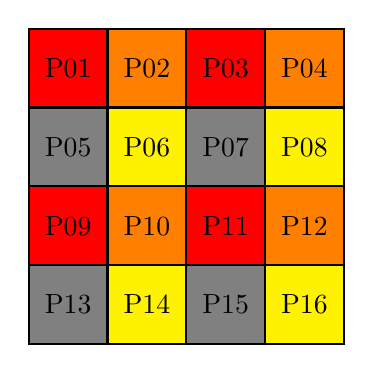
\begin{tikzpicture}
		    [%%%%%%%%%%%%%%%%%%%%%%%%%%%%%%
		        box/.style={rectangle,draw=black,thick, minimum size=1cm},
		    ]%%%%%%%%%%%%%%%%%%%%%%%%%%%%%%
		\draw[step=1cm,color=gray] (-2,-2) grid (2,2);
		\node[box, fill=red] at (-1.5,+1.50) {P01};
		\node[box, fill=orange] at (-0.50,+1.50) {P02};
		\node[box, fill=red] at (+0.50,+1.50) {P03};
		\node[box, fill=orange] at (+1.5,+1.50) {P04};

		\node[box, fill=gray] at (-1.5,+0.50) {P05};
		\node[box, fill=yellow] at (-0.50,+0.50) {P06};
		\node[box, fill=gray] at (+0.50,+0.50) {P07};
		\node[box, fill=yellow] at (+1.50,+0.50) {P08};

		\node[box, fill=red] at (-1.50,-0.50) {P09};
		\node[box, fill=orange] at (-0.50,-0.50) {P10};
		\node[box, fill=red] at (+0.50,-0.50) {P11};
		\node[box, fill=orange] at (+1.50,-0.50) {P12};

		\node[box, fill=gray] at (-1.50,-1.50) {P13};
		\node[box, fill=yellow] at (-0.50,-1.50) {P14};
		\node[box, fill=gray] at (+0.50,-1.50) {P15};
		\node[box, fill=yellow] at (+1.50,-1.50) {P16};
		\end{tikzpicture}
	\end{subfigure}
	{\LARGE$\xrightarrow{FourCombine}$}
	\begin{subfigure}[b]{0.27\textwidth}
		\centering
		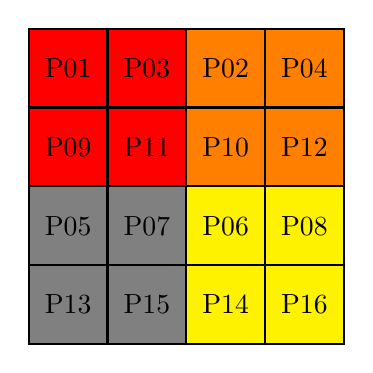
\begin{tikzpicture}
		    [%%%%%%%%%%%%%%%%%%%%%%%%%%%%%%
		        box/.style={rectangle,draw=black,thick, minimum size=1cm},
		    ]%%%%%%%%%%%%%%%%%%%%%%%%%%%%%%
		\draw[step=1cm,color=gray] (-2,-2) grid (2,2);
		\node[box, fill=red] at (-1.5,+1.50) {P01};
		\node[box, fill=red] at (-0.50,+1.50) {P03};
		\node[box, fill=orange] at (+0.50,+1.50) {P02};
		\node[box, fill=orange] at (+1.5,+1.50) {P04};

		\node[box, fill=red] at (-1.5,+0.50) {P09};
		\node[box, fill=red] at (-0.50,+0.50) {P11};
		\node[box, fill=orange] at (+0.50,+0.50) {P10};
		\node[box, fill=orange] at (+1.50,+0.50) {P12};

		\node[box, fill=gray] at (-1.50,-0.50) {P05};
		\node[box, fill=gray] at (-0.50,-0.50) {P07};
		\node[box, fill=yellow] at (+0.50,-0.50) {P06};
		\node[box, fill=yellow] at (+1.50,-0.50) {P08};

		\node[box, fill=gray] at (-1.50,-1.50) {P13};
		\node[box, fill=gray] at (-0.50,-1.50) {P15};
		\node[box, fill=yellow] at (+0.50,-1.50) {P14};
		\node[box, fill=yellow] at (+1.50,-1.50) {P16};

		\end{tikzpicture}
	\end{subfigure}
	\caption{Distribución de píxeles tras aplicar el filtro de combinar}
	\label{fourCombine_transform}
\end{figure}

También podemos ver en la figura~\ref{fourCombine_example} cual es el impacto de nuestro filtro en una imagen real, podremos notar aquí lo parecidas que son imágenes resultantes en cada uno de los cuadrantes, a nuestro ojo es casi imperceptible la diferencia.

\begin{figure}[H]
	\centering
	$\vcenter{\hbox{\includegraphics[scale=0.38]{img/fourCombine_before.jpg}}}$
	$\vcenter{\hbox{\LARGE$\xrightarrow{\text{T}}$}}$
	$\vcenter{\hbox{\includegraphics[scale=0.38]{img/fourCombine_after.jpg}}}$

	\caption{Imagen real antes y luego de la aplicación del filtro}
	\label{fourCombine_example}
\end{figure}

\subsection{Implementación}
\paragraph{Solución en código C}
La solución que fue planteada en c consiste en recorrer la matriz asociada a la imagen de entrada una sola vez píxel por píxel. Cada uno de estos píxeles posee una coordenada y por medio de esta se calcula la coordenada en la matriz asociada a la imagen de salida. 


\paragraph{Solución en ASM}
En cuanto a la implementación en código assembler se tuvo que pensar una solución totalmente diferente ya que al tener que hacerlo con registros de 128 bits nuestra solución de agarrar los píxeles uno por uno y calcular su lugar correspondiente no seria posible. Se tomaron las siguientes decisiones de modelado Decisiones de modelado:
\begin{itemize}
\item Decidir con cuanta información a la vez íbamos a trabajar , se llego a la conclusión que lo mejor seria trabajar con 8 píxeles a la vez. Esta decisión se tomo puesto que eligiendo los 8 píxeles del lugar correcto podíamos llegar a armar 8 píxeles que iban a ser puestos en la imagen de salida. Esto nos debería dar un ahorro en la cantidad de veces que vamos a pegarle a memoria.
\item Decidir entre la posibilidad de agarrar 16 píxeles que este en la misma fila o que estén la misma columna. Nos pareció lo mas fácil de implementar y lo mas efectivo a la hora de usar la cache era que tomáramos 8 píxeles contiguos. Se vera mas adelante en un experimento la diferencia entre ambos
\item Ya que íbamos a tomar de a 8 píxeles contiguos pero el enunciado del trabajo practico solo aseguraba que la imagen a lo ancho iba a ser múltiplo de 4 , teníamos que hacer algo con respecto a los casos donde la imagen no era múltiplo de 8. En este caso tratamos de emular un poco la practica que realiza muchas veces el compilador de intel donde este separa el código en casos especiales para poder ahorrarse de preguntar en el medio del código . Por ende en nuestro código ASM solo preguntamos una vez si el ancho es múltiplo de 4 o de 8 y dependiendo de eso el código se disfurca en dos
\end{itemize}

Ahora hablemos un poco mas de la iteración dentro del un ciclo de nuestro código ASM , podemos separar lo que hace dentro de una columna de lo que hace al cambiar de fila. Dentro de una columna nuestro objetivo es agarrar 8 píxeles desde el puntero $RDI$, agarrando primero cuatro y guardarlo en $XMM2, XMM4$ , moverse y agarrar cuatro mas y guardarlo en $XMM3, XMM5$ llámense $Pi$ con $1\leq i\leq 8$ y trabajarlos de forma tal que queden listos para ser pegados en la memoria de la imagen destino. El siguiente gráfico nos mostrara como ocurre la transformación de los 8 píxeles desde que son extraídos desde la imagen fuente hasta que están listos para ser puestos en la imagen destino : 

\begin{center}
	\begin{tikzpicture}
		\matrix [matrix of nodes,row sep=,row sep=0mm,
		column 1/.style={nodes={rectangle,draw,minimum width=3em}},
		column 2/.style={nodes={rectangle,draw,minimum width=3em}},
		column 3/.style={nodes={rectangle,draw,minimum width=3em}},
		column 4/.style={nodes={rectangle,draw,minimum width=3em}},
		] (P)
		{
		P8 & P7 & P6 & P5\\
		};
	\end{tikzpicture}
	\begin{tikzpicture}
		\matrix [matrix of nodes,row sep=,row sep=0mm,
		column 1/.style={nodes={rectangle,draw,minimum width=3em}},
		column 2/.style={nodes={rectangle,draw,minimum width=3em}},
		column 3/.style={nodes={rectangle,draw,minimum width=3em}},
		column 4/.style={nodes={rectangle,draw,minimum width=3em}},
		] (P)
		{
		P4 & P3 & P2 & P1\\
		};
	\end{tikzpicture}
\end{center}

Separo en pares e impares

\begin{center}
	\begin{tikzpicture}
	\matrix [matrix of nodes,row sep=,row sep=0mm,
	column 1/.style={nodes={rectangle,draw,minimum width=3em}},
	column 2/.style={nodes={rectangle,draw,minimum width=3em}},
	column 3/.style={nodes={rectangle,draw,minimum width=3em}},
	column 4/.style={nodes={rectangle,draw,minimum width=3em}},
	] (P)
	{
	0 & P7 & 0 & P5\\
	};
	\end{tikzpicture}
	\begin{tikzpicture}
	\matrix [matrix of nodes,row sep=,row sep=0mm,
	column 1/.style={nodes={rectangle,draw,minimum width=3em}},
	column 2/.style={nodes={rectangle,draw,minimum width=3em}},
	column 3/.style={nodes={rectangle,draw,minimum width=3em}},
	column 4/.style={nodes={rectangle,draw,minimum width=3em}},
	] (P)
	{
	0 & P3 & 0 & P1\\
	};
	\end{tikzpicture}

	\begin{tikzpicture}
	\matrix [matrix of nodes,row sep=,row sep=0mm,
	column 1/.style={nodes={rectangle,draw,minimum width=3em}},
	column 2/.style={nodes={rectangle,draw,minimum width=3em}},
	column 3/.style={nodes={rectangle,draw,minimum width=3em}},
	column 4/.style={nodes={rectangle,draw,minimum width=3em}},
	] (P)
	{
	P8 & 0 & P6 & 0\\
	};
	\end{tikzpicture}
	\begin{tikzpicture}
	\matrix [matrix of nodes,row sep=,row sep=0mm,
	column 1/.style={nodes={rectangle,draw,minimum width=3em}},
	column 2/.style={nodes={rectangle,draw,minimum width=3em}},
	column 3/.style={nodes={rectangle,draw,minimum width=3em}},
	column 4/.style={nodes={rectangle,draw,minimum width=3em}},
	] (P)
	{
	P4 & 0 & P2 & 0\\
	};
	\end{tikzpicture}
\end{center}

Shifteo pre juntar

\begin{center}
	\begin{tikzpicture}
	\matrix [matrix of nodes,row sep=,row sep=0mm,
	column 1/.style={nodes={rectangle,draw,minimum width=3em}},
	column 2/.style={nodes={rectangle,draw,minimum width=3em}},
	column 3/.style={nodes={rectangle,draw,minimum width=3em}},
	column 4/.style={nodes={rectangle,draw,minimum width=3em}},
	] (P)
	{
	P7 & 0 & P5 & 0\\
	};
	\end{tikzpicture}
	\begin{tikzpicture}
	\matrix [matrix of nodes,row sep=,row sep=0mm,
	column 1/.style={nodes={rectangle,draw,minimum width=3em}},
	column 2/.style={nodes={rectangle,draw,minimum width=3em}},
	column 3/.style={nodes={rectangle,draw,minimum width=3em}},
	column 4/.style={nodes={rectangle,draw,minimum width=3em}},
	] (P)
	{
	0 & P4 & 0 & P2\\
	};
	\end{tikzpicture}
\end{center}

Los uno cruzados con un or

\begin{center}
	\begin{tikzpicture}
	\matrix [matrix of nodes,row sep=,row sep=0mm,
	column 1/.style={nodes={rectangle,draw,minimum width=3em}},
	column 2/.style={nodes={rectangle,draw,minimum width=3em}},
	column 3/.style={nodes={rectangle,draw,minimum width=3em}},
	column 4/.style={nodes={rectangle,draw,minimum width=3em}},
	] (P)
	{
	P7 & P3 & P5 & P1\\
	};
	\end{tikzpicture}
	\begin{tikzpicture}
	\matrix [matrix of nodes,row sep=,row sep=0mm,
	column 1/.style={nodes={rectangle,draw,minimum width=3em}},
	column 2/.style={nodes={rectangle,draw,minimum width=3em}},
	column 3/.style={nodes={rectangle,draw,minimum width=3em}},
	column 4/.style={nodes={rectangle,draw,minimum width=3em}},
	] (P)
	{
	P8 & P4 & P6 & P2\\
	};
	\end{tikzpicture}
\end{center}

Hago shuffle 

\begin{center}
	\begin{tikzpicture}
	\matrix [matrix of nodes,row sep=,row sep=0mm,
	column 1/.style={nodes={rectangle,draw,minimum width=3em}},
	column 2/.style={nodes={rectangle,draw,minimum width=3em}},
	column 3/.style={nodes={rectangle,draw,minimum width=3em}},
	column 4/.style={nodes={rectangle,draw,minimum width=3em}},
	] (P)
	{
	P7 & P5 & P3 & P1\\
	};
	\end{tikzpicture}
	\begin{tikzpicture}
	\matrix [matrix of nodes,row sep=,row sep=0mm,
	column 1/.style={nodes={rectangle,draw,minimum width=3em}},
	column 2/.style={nodes={rectangle,draw,minimum width=3em}},
	column 3/.style={nodes={rectangle,draw,minimum width=3em}},
	column 4/.style={nodes={rectangle,draw,minimum width=3em}},
	] (P)
	{
	P8 & P6 & P4 & P2\\
	};
	\end{tikzpicture}
\end{center}

Una vez que tenemos los 8 píxeles ordenados según los quiero procedo a guardarlos en la posiciones de memoria a las que apuntan el registro $R8$ y $R9$ sin preocuparme en este caso del cuadrante donde estos dos están apuntando. Ya que podrian estar apuntando a un lugar del cuadrante 1, 2 o bien podria ser 3, 4. Pasare a mostrar que ocurre con los registros R8, R9, R10, R11 durante el primer ciclo de columna y luego de haber cambiado de fila. 

Aqui una imagen intentado mostrar el cambio de estado de los registros : 

\begin{figure}[H]
	\centering
	\begin{subfigure}[b]{0.27\textwidth}
		\centering
		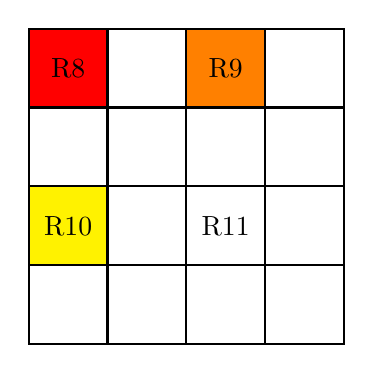
\begin{tikzpicture}
		    [%%%%%%%%%%%%%%%%%%%%%%%%%%%%%%
		        box/.style={rectangle,draw=black,thick, minimum size=1cm},
		    ]%%%%%%%%%%%%%%%%%%%%%%%%%%%%%%
		\draw[step=1cm,color=gray] (-2,-2) grid (2,2);
		\node[box, fill=red] at (-1.5,+1.50) {R8};
		\node[box] at (-0.50,+1.50) {};
		\node[box, fill=orange] at (+0.50,+1.50) {R9};
		\node[box] at (+1.5,+1.50) {};
		\node[box] at (-1.5,+0.50) {};
		\node[box] at (-0.50,+0.50) {};
		\node[box] at (+0.50,+0.50) {};
		\node[box] at (+1.50,+0.50) {};
		\node[box, fill=yellow] at (-1.50,-0.50) {R10};
		\node[box] at (-0.50,-0.50) {};
		\node[box] at (+0.50,-0.50) {R11};
		\node[box] at (+1.50,-0.50) {};
		\node[box] at (-1.50,-1.50) {};
		\node[box] at (-0.50,-1.50) {};
		\node[box] at (+0.50,-1.50) {};
		\node[box] at (+1.50,-1.50) {};
		\end{tikzpicture}
	\end{subfigure}
	{\LARGE$\xrightarrow{Luego de Ciclo Columna}$}
	\begin{subfigure}[b]{0.27\textwidth}
		\centering
		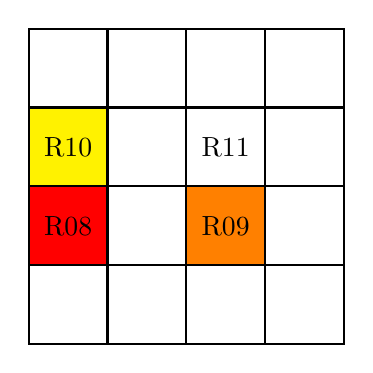
\begin{tikzpicture}
		    [%%%%%%%%%%%%%%%%%%%%%%%%%%%%%%
		        box/.style={rectangle,draw=black,thick, minimum size=1cm},
		    ]%%%%%%%%%%%%%%%%%%%%%%%%%%%%%%
		\draw[step=1cm,color=gray] (-2,-2) grid (2,2);
		\node[box] at (-1.5,+1.50) {};
		\node[box] at (-0.50,+1.50) {};
		\node[box] at (+0.50,+1.50) {};
		\node[box] at (+1.5,+1.50) {};

		\node[box, fill=yellow] at (-1.5,+0.50) {R10};
		\node[box] at (-0.50,+0.50) {};
		\node[box] at (+0.50,+0.50) {R11};
		\node[box] at (+1.50,+0.50) {};

		\node[box, fill=red] at (-1.50,-0.50) {R08};
		\node[box] at (-0.50,-0.50) {};
		\node[box, fill=orange] at (+0.50,-0.50) {R09};
		\node[box] at (+1.50,-0.50) {};

		\node[box] at (-1.50,-1.50) {};
		\node[box] at (-0.50,-1.50) {};
		\node[box] at (+0.50,-1.50) {};
		\node[box] at (+1.50,-1.50) {};

		\end{tikzpicture}
	\end{subfigure}
	\caption{Lugar que ocupan los registros $R8,R9,R10,R11$ antes y luego del cambio de fila}
	\label{fourCombine_rowchange}
\end{figure}

En cuando a que pasa cuando la iteración sobre la columna se termina y se pasa a una nueva fila se realizan lo siguiente :
\begin{itemize}

\item El R8 toma el valor de R9

\item El valor de R9 se el valor de la mitad de una fila 

\item Se switchea R8 R9 por R10 R11 reespectivamente
\end{itemize}

Snippet del código del switch:

\begin{lstlisting}
	mov rax, r8
	mov r8, r10
	mov r10, rax
	mov rax, r9
	mov r9, r11
	mov r11, rax
\end{lstlisting}

Lo único que cambia de esta explicación con respecto a cuando el ancho no es multiplo de 8 es en este punto donde tenemos que cambiar de fila, ya que nos quedaron 4 píxeles sin procesar y como seria demasiado trabajoso holdearlos para poder trabajarlos en otra iteración posterior, lo mejor que nos ocurrió fue trabajarlos manualmente e insertarlos en el lugar donde les corresponde. Luego de esto se sigue con el paso recién explicado.


\subsection{Análisis preliminar}

\begin{center}
	\includegraphics[scale=0.5]{img/fourCombine_CvsASMvsO3.png}
\end{center}

Al igual que los conversores, el tiempo de ejecución del filtro es una función lineal del tamaño de la imagen en pixeles. Este comportamiento era esperado, ya que los mismos solo deben moverse a la memoria destino, lo cual es una operación de tiempo constante.

Nuevamente, algunas mediciones con imágenes más pequeñas tienen ruido visible, pero la pendiente de crecimiento del gráfico se mantiene.

\begin{center}
	\includegraphics[scale=0.5]{img/fourCombine_CvsASMvsO3_bars.png}
\end{center}

En términos de performance, podemos ver que la versión implementada con SSE opera en aproximadamente 45\% del tiempo que la versión optimizada de C.


Para este caso particular, decidimos analizar el ensamblador generado por \texttt{gcc} tanto para \texttt{-O0} como para \texttt{-O3}. Para esto usamos la herramienta Compiler Explorer (\url{https://godbolt.org/}), que nos permitió analizar el código y sus cambios en vivo, asociando cada linea de código C con su correspondiente en ASM.

Una linea en particular que nos llamó la atención fue la siguiente

\begin{lstlisting}
		mDst[offsetH + (h >> 1)][offsetW + (w >> 1)] = mSrc[h][w];
\end{lstlisting}

Cuando no se activa ninguna optimización, $h >> 1$ se calcula cada vez que se necesita, en cada iteración del ciclo. En cambio, al activar las optimizaciones, ese valor se calcula y almacena antes de comenzar el ciclo. Existen otras mejoras pero el nivel del código no nos permitió apreciar grandes diferencias.

\subsection{Experimentación}


\subsubsection*{Hipótesis 1: cargar 16 pixeles a la vez mejora la performance}
Tratamos de llevar a cabo en este conjunto de experimentación la idea de Loop unrolling , con alguna pequeña modificación. Si vamos a lo que se entiende como Loop unrolling no lo podríamos aplicar a la solución presentada ya que este sirve para cuando existe una cantidad finita de iteraciones en realidad lo que se realizo fue el unroll de un ciclo logrando asi reducir la cantidad de ciclos a la mitad. Pasamos a procesar 16 pixeles a la vez pero distribuidos en dos filas , de esta manera solo habría que tener en cuenta que las filas sean múltiplos de 2 es decir pares para poder aplicar esta mejora al algoritmo.

A la hora de ver que tipo de experimentos hacíamos evaluamos dos aspectos:
\begin{itemize}
\item Ver bien de cerca que es lo que pasa con nuestras dos implementaciones porque si tomamos las medidas en una escala muy chica vamos a perder información sobre que lo que esta pasando. 

\item También nos gustaría saber cual es el tiempo que se demoran ambos algoritmos en desarrollar un ciclo. Sabemos que la diferencia esta en que ambos resuelven diferente cantidad de  píxeles a la vez, por ende el tiempo que demoren en resolver un ciclo va a estar dividido por la cantidad de elementos que trabaja a la vez. Vamos a poner también en la misma linea el tiempo de un ciclo del algoritmo de c que solo procesa un píxel a la vez.
\end{itemize}
\begin{figure}[H]
	\centering
	\includegraphics[scale=0.5]{img/fourCombine_UnrollvsNormal.png}
	\caption{Versión Unroll del algoritmo puesta en comparación del entregado como respuesta del tp}
	\label{fourCombine_unroolvsnormal}
\end{figure}

\begin{figure}[H]
	\centering
	\includegraphics[scale=0.5]{img/fourCombine_UnrollvsNormal_asmOnly.png}
	\caption{Comparación exclusiva de las implementaciones en ASM}
	\label{fourCombine_unroolvsnormal_asmOnly}
\end{figure}

\begin{figure}[H]
	\centering
	\includegraphics[scale=0.5]{img/fourCombine_ticks_en_ciclo.png}
	\caption{Ticks en un ciclo comparación de las 3 implementaciones}
	\label{fourCombine_ticksciclo}
\end{figure}

Podemos distinguir de la figura~\ref{fourCombine_unroolvsnormal} que hay una mejora a medida que la imagen se va haciendo cada vez mas grande en el algoritmo de desarrollo del ciclo, esto nos estaría indicando a simple vista que el método funciona, podríamos tener alguna desventaja ya que nuestro programa estaría pesando mas de lo normal, pero esto no sería algo que tenga importancia en un programa como el desarrollado. También se puede hablar de la comparación en imágenes chicas viendo la figura~\ref{fourCombine_unroolvsnormal_asmOnly} . En este caso se trabajo con los resultados mas chicos del set de resultados para poder ver que tan distintos o iguales eran los algoritmos y se puede notar que en imágenes chicas no hay casi diferencia de performance, esto tiene sentido pensando que en imágenes chicas no existe una cantidad de saltos que pueda llegar a influir en la predicción de saltos del procesador.

Por ultimo en la figura~\ref{fourCombine_ticksciclo} una manera interesante de ver la diferencia de la performance que se nos ocurrió fue la de medir un ciclo de cada algoritmo y dividirlo por la cantidad de pixeles que procesan en ese ciclo y asi ver que tan performante era cada uno luego de hacer la modificación a esto como se indica en la sección de "como y que van a medir" se puede observar otra manera como la implementación de UNROLL lograr obtener un tiempo que es al menos dos veces mejor que el método puesto en nuestro TP. Este resultado parece contradecir los anteriores dos ya que en estos no se observa que los resultados del UNROLL sean dos veces mejores. No fue testeado pero mi hipótesis recae a que el trabajo que se debe hacer cada vez que se cambia de fila es mayor cuando estamos haciendo el UNROLL , tal vez por la misma ineficiencia de la implementación. Pero este resultado nos muestra el potencial que tiene el UNROLL al poder tener un mejor tiempo de procesamiento por píxel.


\subsubsection*{Hipótesis 2: usar registro AVX mejora la performance}
Otra idea que había surgido para probar en un experimento fue la de usar registros mas grandes (AVX) para poder lograr así una reducción a la hora de mezclar los elementos, se había pensado que teniendo muchos mas píxeles juntos iba a resultar mas fácil poder ordenarlos para su posterior puesta en en memoria. El problema con este experimento fue que encontramos que las instrucciones AVX (que funcionan en 256 bits) lo único que hacen es replicar comportamientos en la parte baja y la alta del registro es decir los trata como dos registros de 128 bits que solo logran comportamientos de este tipo de registro. Desistimos de hacer este experimento por no encontrar las instrucciones necesarias para poder realizar un código mas performante que el propuesto como solución.

\subsubsection*{Hipótesis 3: el código presentado hace buen uso de la memoria cache}
Nos propusimos ademas cambiar el código para lograr así demostrar que nuestro algoritmo presentado al leer fila por fila logra una mejora en cuando a la administración de la memoria cache. 

Los cambios en el código para lograr esto fueron:
\begin{itemize}
\item En vez de procesar los pixeles fila por fila lo hicimos columna por columna. De esta forma esperamos que en imágenes grande la cantidad de misses en la memoria cache 

\item Procesar la misma cantidad de pixeles por ciclo en ambas soluciones. Asi podemos evitar dudar de los resultados y pensar en la mejora de uno por sobre la otra por la cantidad de pixeles que esta procesando.

\item Hay un incremento en la cantidad de veces que se pide a la memoria información ya que cada vez que procesamos una columna queremos volver a un estado donde mis punteros estén al principio. Esto puede ayudar a que en casos donde la imagen en su totalidad entra en la cache, se mejore la performance. 
\end{itemize}
\begin{figure}[H]
	\centering
	\includegraphics[scale=0.5]{img/fourCombine_antiCache.png}
	\caption{Procesar por filas de la imagen en contra de procesar en columnas}
	\label{fourCombine_antiCache}
\end{figure}

Aunque quisimos encontrar una mejor manera de poder mostrar lo resultados, espero se pueda apreciar que hasta cierto tamaño de imagen en nuestro caso especifico probamos que en una imagen de tamaño menor a  $128x128p$ la cache no cumple ningun roll y nuestros resultados se parecen bastante. En cambio en imágenes donde la cantidad de pixeles es superior a esta la cache empieza tomar un roll mas importante y se empieza a notar como el algoritmo que presentamos es mucho mas eficiente que el usamos para nuestra experimentación.

\subsection{Trabajos Futuros}
Un experimento interesante que debería estar incluido en el tp sería poder medir que porcentaje de un ciclo del algoritmo presentado como respuesta se utiliza cargando datos, que porcentaje en procesarlos y que porcentaje en cargarlos nuevamente a memoria, tenemos la impresión que la gran mayoría del tiempo se la pasa cargando y poniendo cosas en memoria por ende si quisiéramos mejorar aun mas nuestro algoritmo podríamos solamente trabajar sobre el porcentaje de procesamiento de los datos. Estaríamos en presencia de un cuello de botella representado por la memoria.

Algo interesante para poder medir mejor la diferencia entre las implementaciones y su función con el cache podría ser medir la cantidad de miss/hits que tienen cada una de las implementaciones asi ver en medidas mas tangibles como funciona cada uno de ellos.
